\documentclass[12pt, a4paper]{book}

\usepackage[T1]{fontenc}
\usepackage[utf8]{inputenc}
\usepackage[charter, cal=cmcal]{mathdesign}
\usepackage[scaled=0.92]{helvet}
\usepackage{geometry}
\geometry{a4paper, top=30mm, bottom=30mm, inner=32mm, outer=25mm, marginparwidth=18mm}

\usepackage{amsmath, amsthm}
\usepackage[version=4]{mhchem}
\usepackage{graphicx}
\usepackage[dvipsnames,svgnames,table]{xcolor}
\usepackage{tikz}
\usetikzlibrary{arrows.meta, shapes.geometric, positioning, calc, backgrounds}
\usepackage{pgfplots}
\pgfplotsset{compat=1.18}
\usepackage{tcolorbox}
\tcbuselibrary{skins, breakable, theorems}
\usepackage{titlesec}
\usepackage{fancyhdr}
\usepackage{enumitem}
\usepackage{booktabs}
\usepackage{array}
\usepackage{multicol}
\usepackage{parskip}
\usepackage{siunitx}
\usepackage{colortbl}
\usepackage[colorlinks=true, linkcolor=BrickRed,
            urlcolor=NavyBlue, citecolor=ForestGreen]{hyperref}

\definecolor{JourneyColor}{HTML}{145A32}
\definecolor{ModuleColor}{HTML}{1E8449}
\definecolor{PuzzleColor}{HTML}{1A5276}
\definecolor{DiscoveryColor}{HTML}{B7950B}
\definecolor{WarningColor}{HTML}{C0392B}
\definecolor{ProblemColor}{HTML}{4A235A}
\definecolor{ReflectColor}{HTML}{117A65}
\definecolor{HistoryColor}{HTML}{6E2F1A}
\definecolor{SBlock}{HTML}{AED6F1}
\definecolor{PBlock}{HTML}{A9DFBF}
\definecolor{DBlock}{HTML}{FAD7A0}
\definecolor{FBlock}{HTML}{F9E79F}
\definecolor{NobleGas}{HTML}{D2B4DE}

\newtcolorbox{puzzlebox}[1][]{enhanced,breakable,
  colback=PuzzleColor!6,colframe=PuzzleColor,fonttitle=\bfseries\sffamily,
  title={The Puzzle},attach boxed title to top left={yshift=-2mm,xshift=6mm},
  boxed title style={colback=PuzzleColor},borderline west={3pt}{0pt}{PuzzleColor},#1}

\newtcolorbox{discoverybox}[1][]{enhanced,breakable,
  colback=DiscoveryColor!8,colframe=DiscoveryColor,fonttitle=\bfseries\sffamily,
  title={Discovery},attach boxed title to top left={yshift=-2mm,xshift=6mm},
  boxed title style={colback=DiscoveryColor},borderline west={3pt}{0pt}{DiscoveryColor},#1}

\newtcolorbox{problembox}[1][]{enhanced,breakable,
  colback=ProblemColor!5,colframe=ProblemColor,fonttitle=\bfseries\sffamily,
  title={Problems},attach boxed title to top left={yshift=-2mm,xshift=6mm},
  boxed title style={colback=ProblemColor},borderline west={3pt}{0pt}{ProblemColor},#1}

\newtcolorbox{deepbox}[1][]{enhanced,breakable,
  colback=JourneyColor!5,colframe=JourneyColor,fonttitle=\bfseries\sffamily,
  title={Deep Problems},attach boxed title to top left={yshift=-2mm,xshift=6mm},
  boxed title style={colback=JourneyColor},borderline west={4pt}{0pt}{JourneyColor},#1}

\newtcolorbox{historybox}[1][]{enhanced,breakable,
  colback=HistoryColor!7,colframe=HistoryColor!60,fonttitle=\bfseries\sffamily\small,
  title={Historical Note},attach boxed title to top left={yshift=-2mm,xshift=6mm},
  boxed title style={colback=HistoryColor!80},#1}

\newtcolorbox{reflectionbox}[1][]{enhanced,breakable,
  colback=ReflectColor!6,colframe=ReflectColor,fonttitle=\bfseries\sffamily,
  title={Reflection},attach boxed title to top left={yshift=-2mm,xshift=6mm},
  boxed title style={colback=ReflectColor},borderline west={3pt}{0pt}{ReflectColor},#1}

\newtcolorbox{namedconcept}[2][]{enhanced,
  colback=ModuleColor!6,colframe=ModuleColor,fonttitle=\bfseries\sffamily\large,
  title={#2},attach boxed title to top left={yshift=-2mm,xshift=6mm},
  boxed title style={colback=ModuleColor},#1}

\newtcolorbox{synthbox}[1][]{enhanced,breakable,
  colback=JourneyColor!8,colframe=JourneyColor!70,fonttitle=\bfseries\sffamily,
  title={Journey 3 Synthesis},attach boxed title to top left={yshift=-2mm,xshift=6mm},
  boxed title style={colback=JourneyColor!70},borderline west={4pt}{0pt}{JourneyColor},#1}

\titleformat{\chapter}[display]
  {\normalfont\sffamily\huge\bfseries\color{JourneyColor}}
  {\textcolor{JourneyColor!60}{\chaptertitlename\ \thechapter}}{10pt}{\Huge}
  [\vspace{2pt}\textcolor{JourneyColor}{\titlerule[1.5pt]}]
\titleformat{\section}
  {\normalfont\sffamily\Large\bfseries\color{ModuleColor}}
  {\thesection}{1em}{}[\textcolor{ModuleColor!40}{\titlerule[0.6pt]}]
\titleformat{\subsection}
  {\normalfont\sffamily\large\bfseries\color{JourneyColor!80}}{\thesubsection}{1em}{}
\titleformat{\subsubsection}
  {\normalfont\sffamily\normalsize\bfseries}{\thesubsubsection}{1em}{}

\pagestyle{fancy}
\fancyhf{}
\fancyhead[LE]{\small\sffamily\textcolor{JourneyColor}{\leftmark}}
\fancyhead[RO]{\small\sffamily\textcolor{ModuleColor}{\rightmark}}
\fancyfoot[C]{\small\thepage}
\renewcommand{\headrulewidth}{0.4pt}

\newcommand{\newterm}[1]{\textit{\textcolor{DiscoveryColor}{#1}}}
\newcommand{\important}[1]{\textcolor{ModuleColor}{\textbf{#1}}}

\begin{document}
\setcounter{chapter}{2}
\chapter[Journey 3 --- The Periodic Table as a Discovery Engine]
        {Journey Three\\[8pt]
         \textcolor{ModuleColor}{\large The Periodic Table as a Discovery Engine}}
\setcounter{section}{4}

\section{Module 3.5 --- Journey 3 Synthesis: The Table as a Prediction Engine}
\label{sec:mod3.5}

\subsection*{Motivation}

This module does not introduce new material.
Instead, it asks you to use everything from Journey~3
--- and indeed from Journeys~1 and 2 ---
to answer a set of increasingly demanding prediction problems.

The periodic table's value is not as a reference.
Its value is as a \emph{reasoning tool}.
Given an element's position, you should be able to predict:
its electron configuration, its oxidation states,
its bonding character, its reactivity, the formulas of its
compounds, its colour, its magnetic behaviour, its radius,
and its ionisation energy.

By the end of this module, you should be able to
use the table the way Mendeleev intended:
as a map that tells you where you are and what
is around the corner.

% ─── The Complete Annotated Table ────────────────────────────────────────────
\subsection{Reading the Full Table}

\begin{center}
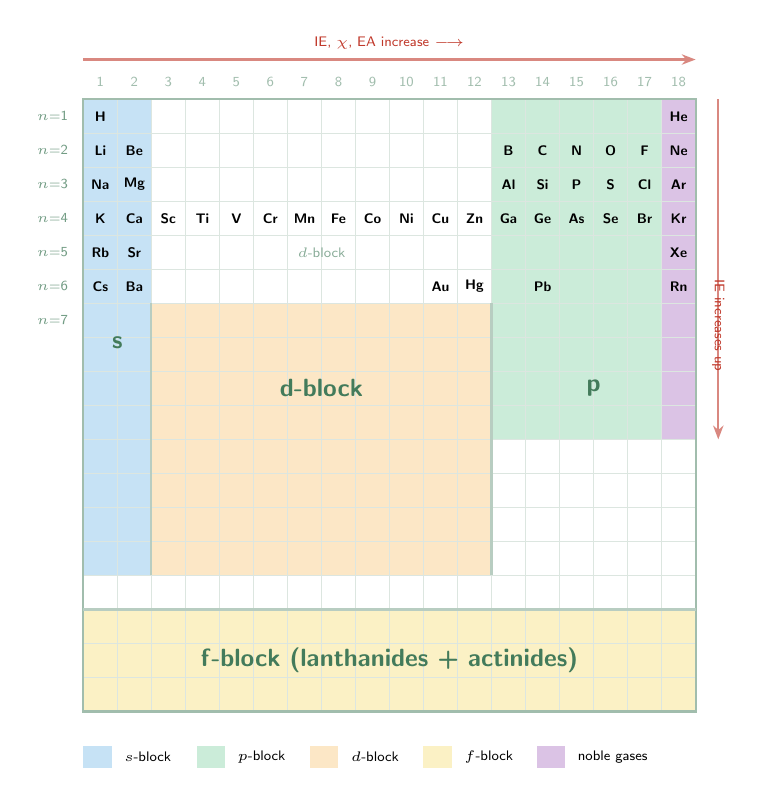
\begin{tikzpicture}[every node/.style={font=\sffamily\footnotesize},
                    scale=0.72]

% ── Block shading ────────────────────────────────────────────────────────────
% s-block: groups 1-2
\fill[SBlock!70]  (0,0) rectangle (1.2, 8.4);
% p-block: groups 13-18
\fill[PBlock!60]  (7.2,2.4) rectangle (10.8, 8.4);
\fill[NobleGas!80] (10.2,2.4) rectangle (10.8, 8.4);
% d-block: groups 3-12, periods 4-7
\fill[DBlock!60]  (1.2,0) rectangle (7.2, 4.8);
% f-block: bottom
\fill[FBlock!60]  (0,-2.4) rectangle (10.8, -0.6);

% ── Grid lines ───────────────────────────────────────────────────────────────
\draw[thin, JourneyColor!15, step=0.6] (0,-2.4) grid (10.8,8.4);

% ── Period labels ────────────────────────────────────────────────────────────
\foreach \p/\y in {1/8.1, 2/7.5, 3/6.9, 4/6.3, 5/5.7, 6/5.1, 7/4.5}{
  \node[left, font=\sffamily\tiny, text=JourneyColor!60] at (-0.1,\y) {$n$=\p};
}

% ── Group labels ─────────────────────────────────────────────────────────────
\foreach \g/\x in {1/0.3, 2/0.9, 3/1.5, 4/2.1, 5/2.7, 6/3.3, 7/3.9,
                   8/4.5, 9/5.1, 10/5.7, 11/6.3, 12/6.9,
                   13/7.5, 14/8.1, 15/8.7, 16/9.3, 17/9.9, 18/10.5}{
  \node[font=\sffamily\tiny, text=JourneyColor!40] at (\x,8.7) {\g};
}

% ── Element cells (selected key elements) ────────────────────────────────────
% Period 1
\node[font=\sffamily\tiny\bfseries] at (0.3,8.1) {H};
\node[font=\sffamily\tiny\bfseries] at (10.5,8.1) {He};
% Period 2
\node[font=\sffamily\tiny\bfseries] at (0.3,7.5) {Li};
\node[font=\sffamily\tiny\bfseries] at (0.9,7.5) {Be};
\foreach \elem/\x in {B/7.5, C/8.1, N/8.7, O/9.3, F/9.9, Ne/10.5}{
  \node[font=\sffamily\tiny\bfseries] at (\x,7.5) {\elem};
}
% Period 3
\node[font=\sffamily\tiny\bfseries] at (0.3,6.9) {Na};
\node[font=\sffamily\tiny\bfseries] at (0.9,6.9) {Mg};
\foreach \elem/\x in {Al/7.5, Si/8.1, P/8.7, S/9.3, Cl/9.9, Ar/10.5}{
  \node[font=\sffamily\tiny\bfseries] at (\x,6.9) {\elem};
}
% Period 4
\node[font=\sffamily\tiny\bfseries] at (0.3,6.3) {K};
\node[font=\sffamily\tiny\bfseries] at (0.9,6.3) {Ca};
\foreach \elem/\x in {Sc/1.5, Ti/2.1, V/2.7, Cr/3.3, Mn/3.9,
                       Fe/4.5, Co/5.1, Ni/5.7, Cu/6.3, Zn/6.9}{
  \node[font=\sffamily\tiny\bfseries] at (\x,6.3) {\elem};
}
\foreach \elem/\x in {Ga/7.5, Ge/8.1, As/8.7, Se/9.3, Br/9.9, Kr/10.5}{
  \node[font=\sffamily\tiny\bfseries] at (\x,6.3) {\elem};
}
% Period 5 (abbreviated)
\node[font=\sffamily\tiny\bfseries] at (0.3,5.7) {Rb};
\node[font=\sffamily\tiny\bfseries] at (0.9,5.7) {Sr};
\node[font=\sffamily\tiny, text=JourneyColor!50] at (4.2,5.7) {$d$-block};
\node[font=\sffamily\tiny\bfseries] at (10.5,5.7) {Xe};
% Period 6 (abbreviated)
\node[font=\sffamily\tiny\bfseries] at (0.3,5.1) {Cs};
\node[font=\sffamily\tiny\bfseries] at (0.9,5.1) {Ba};
\foreach \elem/\x in {Au/6.3, Hg/6.9, Pb/8.1}{
  \node[font=\sffamily\tiny\bfseries] at (\x,5.1) {\elem};
}
\node[font=\sffamily\tiny\bfseries] at (10.5,5.1) {Rn};

% ── Block labels ─────────────────────────────────────────────────────────────
\node[font=\sffamily\small\bfseries, text=JourneyColor!80] at (0.6,4.1)
  {\textit{s}};
\node[font=\sffamily\small\bfseries, text=JourneyColor!80] at (4.2,3.3)
  {\textit{d}-block};
\node[font=\sffamily\small\bfseries, text=JourneyColor!80] at (9.0,3.3)
  {\textit{p}};
\node[font=\sffamily\small\bfseries, text=JourneyColor!80] at (5.4,-1.5)
  {\textit{f}-block (lanthanides + actinides)};

% ── Trend arrows ─────────────────────────────────────────────────────────────
\draw[-{Stealth[length=5pt]}, thick, WarningColor!60]
  (11.2,8.4) -- (11.2,2.4)
  node[right, midway, font=\sffamily\tiny, text=WarningColor, rotate=270]
    {IE increases up};
\draw[-{Stealth[length=5pt]}, thick, WarningColor!60]
  (0,9.1) -- (10.8,9.1)
  node[above, midway, font=\sffamily\tiny, text=WarningColor]
    {IE, $\chi$, EA increase $\longrightarrow$};

% ── Outer border ─────────────────────────────────────────────────────────────
\draw[thick, JourneyColor!40] (0,-2.4) rectangle (10.8,8.4);
\draw[thick, JourneyColor!30] (0,-0.6) -- (10.8,-0.6);
\draw[thick, JourneyColor!30] (1.2,0) -- (1.2,4.8);
\draw[thick, JourneyColor!30] (7.2,0) -- (7.2,4.8);

% ── Legend ───────────────────────────────────────────────────────────────────
\fill[SBlock!70]  (0,-3.4) rectangle (0.5,-3.0);
\node[right, font=\sffamily\tiny] at (0.55,-3.2) {$s$-block};
\fill[PBlock!60]  (2.0,-3.4) rectangle (2.5,-3.0);
\node[right, font=\sffamily\tiny] at (2.55,-3.2) {$p$-block};
\fill[DBlock!60]  (4.0,-3.4) rectangle (4.5,-3.0);
\node[right, font=\sffamily\tiny] at (4.55,-3.2) {$d$-block};
\fill[FBlock!60]  (6.0,-3.4) rectangle (6.5,-3.0);
\node[right, font=\sffamily\tiny] at (6.55,-3.2) {$f$-block};
\fill[NobleGas!80] (8.0,-3.4) rectangle (8.5,-3.0);
\node[right, font=\sffamily\tiny] at (8.55,-3.2) {noble gases};

\end{tikzpicture}
\end{center}

\vspace{0.5em}

\subsection{The Prediction Framework}

Before solving any prediction problem, run through
this checklist:

\begin{namedconcept}{The Position-to-Properties Checklist}
Given an element at position (Period $n$, Group $g$, Block $b$):

\begin{enumerate}[nosep, leftmargin=2em]
  \item \textbf{Electron config}: period = outer $n$;
        group (for $s$/$p$) = valence electrons;
        block = subshell being filled.
  \item \textbf{Oxidation states}: $s$-block: group number only.
        $p$-block: group$-$10 to group (usually).
        $d$-block: +2 always, plus higher states from $d$ electrons.
  \item \textbf{Metallic character}: left/lower = metallic.
        Right/upper = nonmetallic.
        Diagonal staircase = metalloids.
  \item \textbf{Atomic radius}: increases left, increases down.
  \item \textbf{Ionisation energy}: increases right, increases up.
  \item \textbf{Electronegativity}: increases right, increases up.
        (F highest; Cs/Fr lowest.)
  \item \textbf{Compound formulas}: determined by valence
        electrons and octet rule.
  \item \textbf{Acid/base of oxide}: metal oxides are basic;
        nonmetal oxides are acidic; metalloid oxides amphoteric.
\end{enumerate}
\end{namedconcept}

\subsection{Prediction Exercises: Working the Table}

\begin{problembox}
\textbf{Predict before you look up.}

For each of the following, make your predictions from
the table alone, then check against real data.

\begin{enumerate}[label=\textbf{\arabic*.}]
  \item \textbf{Tellurium} (Te, $Z=52$, Period 5, Group 16).
        \begin{enumerate}[label=(\alph*)]
          \item Write the electron configuration.
          \item List the most common oxidation states.
          \item Predict whether \ce{TeO2} is acidic or basic.
          \item Predict whether Te is a metal, nonmetal,
                or metalloid.
          \item Predict whether H$_2$Te has a higher or
                lower boiling point than H$_2$S.
                (Hint: think about molecular size and
                London dispersion forces.)
          \item Compare Te to its group congeners O, S, Se:
                which periodic trend dominates the
                acid strength of H$_2$X across the group?
        \end{enumerate}

  \item \textbf{Palladium} (Pd, $Z=46$, Period 5, Group 10).
        \begin{enumerate}[label=(\alph*)]
          \item Write the electron configuration.
                (Note: Pd is anomalous: $[Kr]\,4d^{10}$, not $4d^8\,5s^2$.)
          \item What does the anomaly tell you about
                $4d^{10}$ stability?
          \item Pd is an important catalyst for C--C
                bond formation (Suzuki, Heck reactions).
                What property of Pd makes it catalytically useful?
          \item Predict whether PdO is more easily
                reduced than FeO.
                (Hint: position in the activity series
                reflects stability of the metal oxide.)
        \end{enumerate}

  \item \textbf{A mystery element.}
        Element X has these properties:
        \begin{itemize}[nosep]
          \item Metallic solid at room temperature
          \item Forms a green ion \ce{X^{3+}} in solution
          \item Forms a purple ion \ce{X^{6+}} (as oxyanion)
                in strongly oxidising conditions
          \item Has 6 unpaired electrons in one of its oxidation states
          \item The oxide in oxidation state +3 is amphoteric
        \end{itemize}
        Identify element X, give its $Z$, and write the
        electron configuration that explains the
        6-unpaired-electron observation.
\end{enumerate}
\end{problembox}

\subsection{The Table Predicts New Materials}

The periodic table is not static.
It is actively used to predict new materials.

\subsubsection{High-entropy Alloys}

Traditional alloys (e.g.\ steel, bronze) are based on one
principal element.
High-entropy alloys (HEAs) mix 5+ elements in roughly equal
proportions.

The idea: position adjacent transition metals
(e.g.\ Co, Cr, Fe, Mn, Ni) in the same region of the
$d$-block, where their atomic radii and electronegativities
are similar enough that the mixture is stable.

The result: materials with exceptional hardness, wear
resistance, and high-temperature strength.
CoCrFeMnNi (the ``Cantor alloy'') was predicted from the
table to form a single-phase solid solution --- confirmed in 2004.

\subsubsection{Rechargeable Batteries}

Lithium-ion batteries require a cathode that can reversibly
intercalate \ce{Li+} ions.
The best cathodes are transition metal oxides:
\ce{LiCoO2}, \ce{LiMnO2}, \ce{LiFePO4}.

The selection criterion comes directly from the table:
\begin{itemize}[nosep, leftmargin=2em]
  \item The metal must have two accessible oxidation states
        (so it can accept/donate electrons during charge/discharge).
  \item The energy gap between the two states must match
        the battery's voltage window.
  \item The structure must be stable over thousands of cycles.
\end{itemize}

The periodic table narrows the search space from 118 elements
to the dozen or so transition metals with the right redox chemistry.

\subsubsection{Photovoltaic Materials}

The most efficient solar cells use \ce{ABX3} perovskite crystals
(e.g.\ \ce{CH3NH3PbI3}).
Pb is in Group 14, Period 6 --- heavy enough for
relativistic effects to tune its band gap to match
the solar spectrum.

The search for lead-free perovskites (replacing toxic Pb)
proceeds by the table: Sn and Ge (Period 4 and 5, Group 14)
are the obvious candidates.

\begin{discoverybox}
\textbf{The table as a materials map.}

Every rectangle in the periodic table represents
not just one element, but a cluster of properties.
The $d$-block transition metals in periods 5--6
(Ru, Rh, Pd, Os, Ir, Pt) are ``platinum group metals'' ---
all share high melting points, low reactivity,
and catalytic activity.
They cluster together because they share similar
electron configurations and $Z_\text{eff}$ values.

When materials scientists design a new catalyst, they
do not search at random.
They use the table's structure to identify candidate
elements with the right redox potential, atomic radius,
and surface adsorption energy --- all encoded in position.

The periodic table is the original database of materials science.
\end{discoverybox}

\subsection*{Journey 3 Synthesis}

\begin{synthbox}
Journey~3 has shown that the periodic table is not a list
of facts but a \emph{derived consequence of quantum mechanics}
with immense predictive power.

\begin{center}
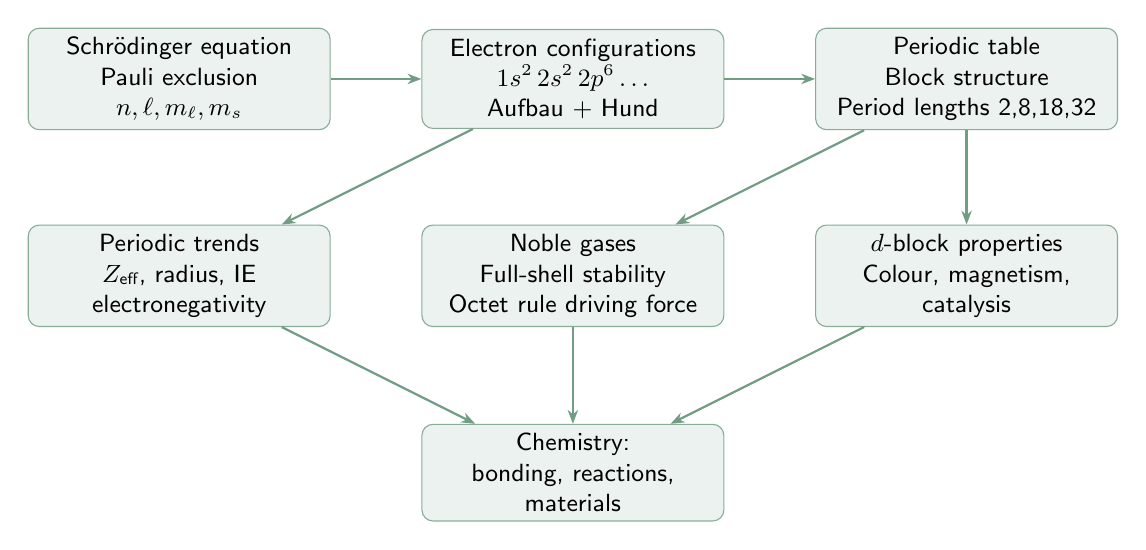
\begin{tikzpicture}[
  every node/.style={font=\sffamily\small, align=center},
  box/.style={draw=JourneyColor!50, fill=JourneyColor!8, rounded corners=4pt,
              minimum width=3.8cm, minimum height=1.0cm, text width=3.6cm},
  arr/.style={-{Stealth[length=5pt]}, thick, JourneyColor!60}
]
  \node[box] (qm)  at (0, 6)
    {Schr\"{o}dinger equation\\Pauli exclusion\\$n,\ell,m_\ell,m_s$};
  \node[box] (ec)  at (5, 6)
    {Electron configurations\\$1s^2\,2s^2\,2p^6\ldots$\\Aufbau + Hund};
  \node[box] (pt)  at (10, 6)
    {Periodic table\\Block structure\\Period lengths 2,8,18,32};
  \node[box] (tr)  at (0, 3.5)
    {Periodic trends\\$Z_\text{eff}$, radius, IE\\electronegativity};
  \node[box] (ng)  at (5, 3.5)
    {Noble gases\\Full-shell stability\\Octet rule driving force};
  \node[box] (dm)  at (10, 3.5)
    {$d$-block properties\\Colour, magnetism,\\catalysis};
  \node[box] (ch)  at (5, 1)
    {Chemistry:\\bonding, reactions,\\materials};

  \draw[arr] (qm) -- (ec);
  \draw[arr] (ec) -- (pt);
  \draw[arr] (ec) -- (tr);
  \draw[arr] (pt) -- (ng);
  \draw[arr] (pt) -- (dm);
  \draw[arr] (tr) -- (ch);
  \draw[arr] (ng) -- (ch);
  \draw[arr] (dm) -- (ch);
\end{tikzpicture}
\end{center}

\medskip
\textbf{The five things Journey~3 established:}
\begin{enumerate}[nosep, leftmargin=2em]
  \item The periodic law (Mendeleev, 1869) is an empirical
        shadow of quantum mechanics.
        Period lengths $2,8,8,18,18,32,32$ count electrons
        in orbital shells.
  \item All periodic trends ($Z_\text{eff}$, radius, IE, $\chi$)
        reduce to one concept: how strongly the nucleus
        holds valence electrons after shielding.
  \item Noble gases are the anchors of the table ---
        full-shell endpoints that drive all other chemistry.
        ``Inert'' is only an approximation.
  \item The $d$-block's partially filled orbitals give
        transition metals unique properties: variable
        oxidation states, colour, magnetism, catalysis.
  \item The table is a prediction engine.
        It has predicted undiscovered elements,
        wrong atomic weights, new groups, new compound types,
        and new materials --- consistently, for 150 years.
\end{enumerate}
\end{synthbox}

\subsection*{Deep Problems}

\begin{deepbox}
\begin{enumerate}[label=\textbf{D\arabic*.}]

  \item \textbf{Designing a battery cathode.}

        You are tasked with finding a transition metal oxide
        \ce{MO2} suitable for a lithium-ion battery cathode.
        Requirements:
        \begin{itemize}[nosep]
          \item M must have two accessible oxidation states
                separated by $\sim 3$--4 eV (to match battery voltage)
          \item M oxide must be stable in air
          \item M should be cheap and non-toxic
        \end{itemize}
        \begin{enumerate}[label=(\alph*)]
          \item Using IE data and the periodic table,
                identify two or three candidate metals M
                from the first transition series
                that meet these criteria.
          \item Manganese is used in \ce{LiMnO2} batteries.
                The relevant redox couple is
                Mn$^{3+}$/Mn$^{4+}$.
                Write the electron configurations of
                Mn$^{3+}$ and Mn$^{4+}$.
          \item One problem with Mn cathodes is the
                Jahn-Teller distortion of Mn$^{3+}$ ($d^4$).
                Explain what configuration causes this
                and how it degrades battery cycle life.
          \item LiFePO$_4$ (LFP batteries, used in many
                electric vehicles) uses Fe$^{2+}$/Fe$^{3+}$.
                What advantages does Fe have over Mn
                from the periodic table perspective?
        \end{enumerate}

  \item \textbf{Diagonal relationships explained.}

        Li resembles Mg; Be resembles Al; B resembles Si.
        These ``diagonal pairs'' share chemical properties
        despite being in different groups and periods.

        \begin{enumerate}[label=(\alph*)]
          \item The key property is \newterm{charge density}
                --- the ratio of charge to ionic radius.
                Calculate the charge densities of Li$^+$
                (radius 76 pm) and Mg$^{2+}$ (radius 72 pm).
          \item Both Li$_2$CO$_3$ and MgCO$_3$ decompose
                to the oxide on heating, while Na$_2$CO$_3$
                does not.
                Explain using charge density and the
                polarisation of the carbonate ion.
          \item Be and Al both form amphoteric oxides
                (dissolve in both acid and base).
                Na$_2$O is purely basic; CO$_2$ is purely acidic.
                Using the charge density argument,
                explain where the amphoteric boundary lies
                and why.
          \item Predict whether Ga (Group 13, Period 4)
                has a diagonal relationship with any
                Group 14 element.
                Identify the partner and describe one
                shared property.
        \end{enumerate}

  \item \textbf{The periodic table and the origin of life.}

        The chemistry of life is built from six main elements:
        H, C, N, O, P, S.
        Trace amounts of a dozen transition metals are also
        essential: Fe, Zn, Cu, Mn, Co, Mo, \ldots

        \begin{enumerate}[label=(\alph*)]
          \item All six main biogenic elements are in
                Periods 1--3.
                What property of Period 1--3 elements
                makes them uniquely suited for building
                stable, complex molecules?
                (Hint: bond strength, orbital overlap,
                multiple bonds.)
          \item Phosphorus (Group 15) is unique in
                forming the P--O--P linkages of DNA/RNA
                and ATP.
                No other Group 15 element does this.
                Using periodic trends, explain why N--O--N
                linkages are not stable and why As--O--As
                is too easily hydrolysed.
          \item The essential trace metals (Fe for
                haemoglobin, Zn for enzyme catalysis,
                Cu for electron transfer) are all
                first-row transition metals.
                Why are second-row transition metals
                (Ru, Pd, Ag) largely absent from
                biochemistry despite similar chemistry?
                (Hint: abundance in Earth's crust, ionic radius.)
          \item Silicon (Si) is the second most abundant
                element in Earth's crust, yet life is
                carbon-based.
                Compare C and Si using periodic trends
                (multiple bonds, chain stability, reaction
                with O and H$_2$O) to explain why
                silicon-based life is chemically unlikely.
        \end{enumerate}

\end{enumerate}
\end{deepbox}

\subsection*{Reflection}

\begin{reflectionbox}
\begin{enumerate}[label=\textbf{R\arabic*.}]
  \item Mendeleev discovered the periodic table in 1869.
        The quantum mechanical explanation arrived in 1926 ---
        57 years later.
        For half a century, chemists used the table
        correctly without knowing why it worked.
        \textbf{Does a tool need to be theoretically grounded
        to be scientifically valid?}
        What does it mean to ``understand'' the periodic table
        --- to know the pattern, or to know the mechanism?

  \item The periodic table has 118 confirmed elements.
        The universe contains roughly 92 naturally occurring ones.
        Synthetic elements (93--118) last microseconds to years.
        \textbf{In what sense is the periodic table complete?}
        Could there be chemistry --- useful, accessible chemistry ---
        beyond element 118?

  \item The six biogenic elements (H, C, N, O, P, S) are
        among the most abundant reactive nonmetals in the universe.
        \textbf{Is it surprising that life uses the most
        abundant reactive elements, or would any chemistry
        sufficiently complex to be ``life'' inevitably
        use the same periodic table positions?}
        Is the chemistry of life a cosmic inevitability
        or an accident of Earth's particular composition?

  \item Looking back across Journey~3:
        Mendeleev's empirical table (1869),
        Moseley's $Z$-ordering (1913),
        quantum mechanical derivation (1926),
        Bartlett's xenon compound (1962),
        high-entropy alloys (2004).
        \textbf{The periodic table is 150 years old and
        still generating new science.}
        What distinguishes a scientific framework that ages
        well from one that doesn't?
\end{enumerate}
\end{reflectionbox}

\vspace{1.5em}
\begin{center}
\begin{tcolorbox}[enhanced,
  colback=JourneyColor!12, colframe=JourneyColor,
  width=0.9\textwidth, arc=4pt]
\centering\sffamily
\textbf{\large Journey 3 Complete: The Periodic Table as a Discovery Engine}\\[8pt]
\small
\begin{tabular}{ll}
Module 3.1 & Mendeleev: order from chaos, gaps, predictions \\
Module 3.2 & Periodic trends: $Z_\text{eff}$, radius, IE, electronegativity \\
Module 3.3 & Noble gases: full shells, Bartlett's breakthrough \\
Module 3.4 & Transition metals: colour, magnetism, catalysis \\
Module 3.5 & Synthesis: the table as a prediction engine \\
\end{tabular}\\[8pt]
\textit{The periodic table is a quantum mechanical truth expressed
in 118 boxes.
Every position encodes a complete chemical identity.
Continue to Journey~4: The Bond --- Why Atoms Stick Together.}
\end{tcolorbox}
\end{center}

\end{document}